\documentclass[tikz,border=10pt]{standalone}
\usepackage{fontspec}
\usepackage{xeCJK}
\setmainfont{Times New Roman}
\setCJKmainfont{Hiragino Sans GB}
\setCJKsansfont{Microsoft YaHei}
\setCJKmonofont{STSong}
\usepackage{amsmath}
\usepackage{tikz}
\usetikzlibrary{arrows.meta,calc,positioning}

\tikzset{
  signal/.style={->, line width=1.2pt, draw=black!80, >=Stealth},
  block/.style={draw=blue!70!black, line width=1.2pt, rectangle, minimum width=2.0cm, minimum height=1.0cm, fill=none},
  sum/.style={
    draw=green!55!black, line width=1.2pt, circle, minimum size=0.56cm, inner sep=0pt, fill=none,
    path picture={
      \draw[green!55!black, line width=0.9pt]
        (path picture bounding box.south west) -- (path picture bounding box.north east)
        (path picture bounding box.north west) -- (path picture bounding box.south east);
    }
  }
}

\begin{document}
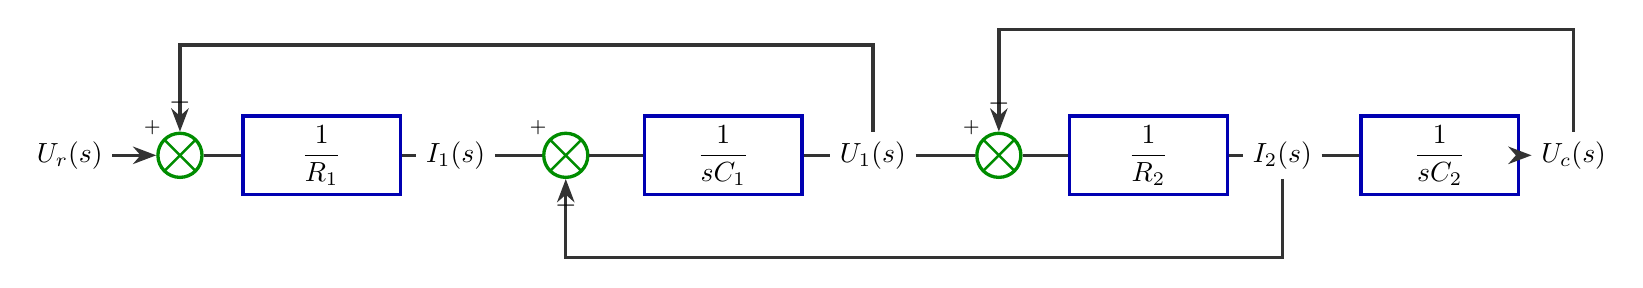
\begin{tikzpicture}[node distance=1.6cm]
  \node (ur) at (0,0) {$U_r(s)$};
  \node[sum] (sum1) at (1.4,0) {};
  \node[block] (r1) at (3.2,0) {$\dfrac{1}{R_1}$};
  \node (i1) at (4.9,0) {$I_1(s)$};
  \node[sum] (sum2) at (6.3,0) {};
  \node[block] (c1) at (8.3,0) {$\dfrac{1}{sC_1}$};
  \node (u1) at (10.2,0) {$U_1(s)$};
  \node[sum] (sum3) at (11.8,0) {};
  \node[block] (r2) at (13.7,0) {$\dfrac{1}{R_2}$};
  \node (i2) at (15.4,0) {$I_2(s)$};
  \node[block] (c2) at (17.4,0) {$\dfrac{1}{sC_2}$};
  \node (uc) at (19.1,0) {$U_c(s)$};

  \draw[signal] (ur) -- (sum1);
  \draw[signal] (sum1) -- (r1) -- (i1) -- (sum2) -- (c1) -- (u1) -- (sum3) -- (r2) -- (i2) -- (c2) -- (uc);

  \draw[signal] (u1) |- ++(0,1.4) -| node[pos=0.95, above] {$-$} (sum1.north);
  \draw[signal] (i2) |- ++(0,-1.3) -| node[pos=0.96, below] {$-$} (sum2.south);
  \draw[signal] (uc) |- ++(0,1.6) -| node[pos=0.96, above] {$-$} (sum3.north);

  \node[font=\scriptsize] at ($(sum1)+(-0.35,0.35)$) {$+$};
  \node[font=\scriptsize] at ($(sum2)+(-0.35,0.35)$) {$+$};
  \node[font=\scriptsize] at ($(sum3)+(-0.35,0.35)$) {$+$};
\end{tikzpicture}
\end{document}
